\documentclass[25pt, a0paper, landscape, cmyk]{tikzposter}
\usepackage[Export]{adjustbox}
\usepackage[colorlinks,allcolors=blue]{hyperref}
\tikzposterlatexaffectionproofoff
\title{One World, One Wiki!}
\author{%
  C. Scott Ananian
  <cananian@wikimedia.org>
  \texttt{[[User:cscott]]}
  (Wikimedia Foundation)
}
%\usetheme{Autumn}\usecolorstyle[colorPalette=BrownBlueOrange]{Britain}
%\usetheme{Envelope}
\usetheme{Rays}\usecolorstyle[colorOne=green,colorTwo=orange]{Australia}
\useinnerblockstyle{Table}
% remove space taken up by \institute
\settitle{ \centering \vbox{
\centering
\color{titlefgcolor} {\bfseries \Huge \sc \@title \par}
\vspace*{1em}
{\huge \@author}
}}

% Work around tikzposter conflict with hyperref
% https://tex.stackexchange.com/questions/254257/tikzposter-and-doi-package-conflict
\def\HyperFirstAtBeginDocument#1{#1}
\begin{document}\maketitle[width=90cm]%[titletextscale=1,width=75cm]
\begin{columns}
  \column{0.5}
  \newlength{\myfigwidth}
  \setlength{\myfigwidth}{0.34\colwidth}
  \newlength{\myfiggap}
  \setlength{\myfiggap}{1.5cm}
  \block{Language Converter}{

    MediaWiki uses
    \href{https://www.mediawiki.org/wiki/Writing_systems\#LanguageConverter}{[[mw:LanguageConverter]]}
    to automatically transliterate articles between closely related
    languages or dialects or script variants of a language or dialect.
    It is used on 11 wikis, and has been requested on about 35 more.
    Here are some examples of conversion pairs:

    \innerblock{%
      \raisebox{0pt}[0pt][0pt]{\parbox{13cm}{\raggedright%
          English (American/British)\\\rm
          \textit{LanguageConverter not used.}

          Spelling and usage differences exist between American
          English, British English, Indian English, and others.
      }}%
    }{%
      \includegraphics[valign=T,width=\myfigwidth]{variants-en-us.eps}%
      \hspace{\myfiggap}%
      \includegraphics[valign=T,width=\myfigwidth]{variants-en-gb.eps}%

      \vspace{1cm}
    }
    \innerblock{
      \raisebox{0pt}[0pt][0pt]{\parbox{13cm}{\raggedright%
          Serbian (Latin/Cyrillic)\\\rm
          \textit{LanguageConverter in use.}

          Speakers are fully functionally digraphic, using both
          Cyrillic and Latin scripts.  There are also vocabulary
          differences between Ikavian, Ekavian, and Ijekavian dialects
          which are not currently converted.
      }}%
    }{%
      \includegraphics[valign=T,width=\myfigwidth]{variants-sr-el.eps}%
      \hspace{\myfiggap}%
      \includegraphics[valign=T,width=\myfigwidth]{variants-sr-ec.eps}%
    }
    \innerblock{
      \raisebox{0pt}[0pt][0pt]{\parbox{13cm}{\raggedright%
          Chinese (Simplified/Traditional)\\\rm
          \textit{LanguageConverter in use.}

          Simplified used in mainland China, Singapore, and
          Malaysia.  Traditional used in Taiwan, Hong Kong,
          Macau, and among Overseas Chinese.
          Most speakers monographic; few can fluently
          proofread text in both variants.
        }}%
    }{%
      \includegraphics[valign=T,width=\myfigwidth]{variants-zh-cn.eps}%
      \hspace{\myfiggap}%
      \includegraphics[valign=T,width=\myfigwidth]{variants-zh-tw.eps}%

      \vspace{7cm}
    }
    \innerblock{
      \raisebox{0pt}[0pt][0pt]{\parbox{13cm}{\raggedright%
          Hindi/Urdu\\\rm
          \textit{LanguageConverter not used.}

          Urdu and Hindi are dialects of the Hindustani language,
          written in very different scripts: Arabic on the Pakistan
          side of the border, Devanagri on the India side.
          (Punjabi is a similar case, with four scripts used.)

          Currently separate small wikis; could combine efforts.
        }}%
    }{%
      \includegraphics[valign=T,width=\myfigwidth]{variants-hi.eps}%
      \hspace{\myfiggap}%
      \includegraphics[valign=T,width=\myfigwidth]{variants-ur.eps}%

      \vspace{3cm}
    }

    %\small LanguageConverter brings our wikis together!
  }
  \column{0.5}
  \block{Native Variant Editing}{

    LanguageConverter is oriented to readers: it converts the article
    text unidirectionally into readable text in a consistent variant.
    But as soon as a user begins to edit, they are confronted with the
    source text in a mix of variants, as illustrated by the
    intermingled Cyrillic and Latin scripts in the article from
    Serbian Wikipedia shown below.  This mixture of scripts can be a
    huge barrier to editing in communities where individuals are
    typically only fluent in a single variant.

    The Parsoid team has been experimenting with a new bidirectional
    implementation of LanguageConverter, based on Finite State
    Transducers (FSTs).  These allow automatic annotation of wikitext
    such that it can be round-tripped to its original variant
    losslessly.  With these annotations, an Wikimedian can edit an
    article in their preferred consistent variant.

    Unedited portions of the article will round-trip to their original
    variant, preventing dirty diffs, and only edited sections will
    reflect the variant which the editor saw.  On wikis where the
    community has chosen to author all articles in a single variant,
    all text can be losslessly saved as the chosen variant, regardless
    of which variant the editor used.

    \begin{center}
    \textbf{We can make editing easier on wikis using LanguageConverter!}
    \end{center}

    \begin{tikzfigure}
      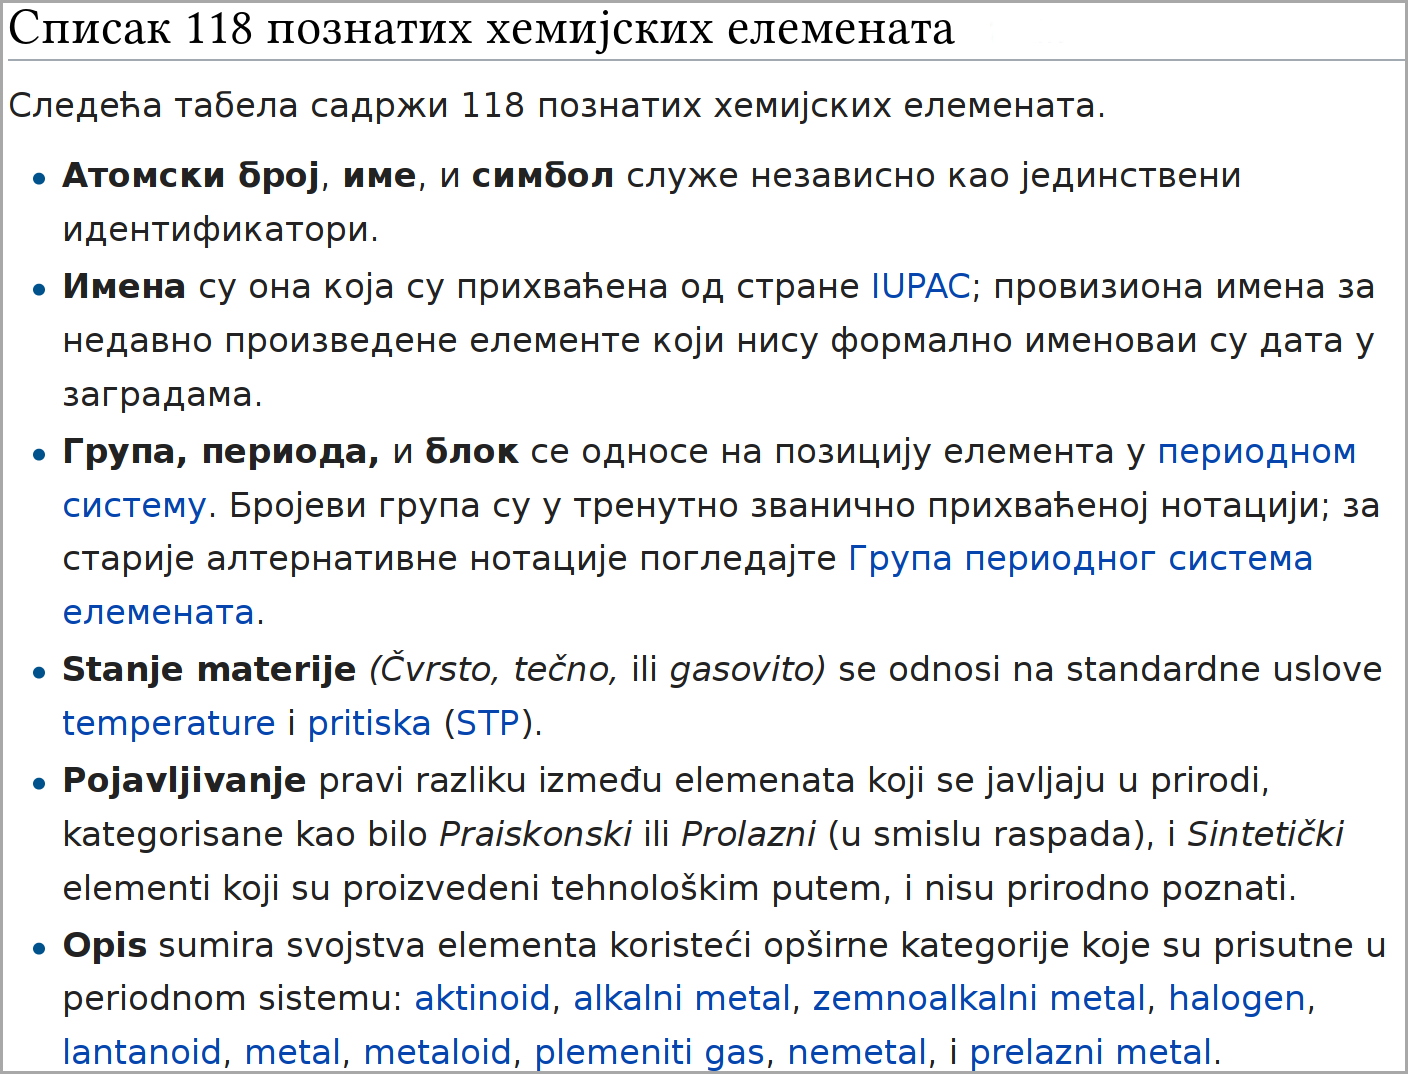
\includegraphics[height=18cm,valign=T]{mixed-edit-2.png}
      \hspace{7cm}
      \includegraphics[height=18cm,valign=T]{simple.eps}

      \vspace{0.75cm}

      \parbox[t]{26cm}{Serbian Wikipedia article showing mixed
        Cyrillic/Latin script}
      \hspace{2cm}
      \parbox[t]{22cm}{Partial FST for Serbian Cyrillic-to-Latin
        conversion}
    \end{tikzfigure}
  }
  \block{Translation Suggestion Tool}{
    lala
  }
  \block{Zero-Shot Translation}{
    lala
  }
\end{columns}
\end{document}
